%\newpage
\subsection{Das Spiel \emph{\gameTitle}}
 ////////////////ändern! gameIntro.tey
Im Spiel \emph{\gameTitle{}} spielen Sie Eins gegen Eins. Jede Person steuert dabei einen Gorilla und versucht den gegnerischen Gorilla mit einer Banane abzuwerfen. Die Gorillas stehen in gewisser Entfernung, einer links und einer rechts, auf verschiedenen Hochh\"ausern einer Skyline. Das Spiel ist rundenbasiert: Zun\"achst t\"atigt der/die erste Spieler\_in den Wurf. Trifft dieser Wurf, so wurde die Runde gewonnen, ansonsten ist der/die n\"achste Spieler\_in an der Reihe. Ein Wurf wird durch zwei Eingaben gesteuert: den Abwurfwinkel und die Wurfgeschwindigkeit. Der Winkel wird als Gradzahl von 0 bis 360 angegeben, die Geschwindigkeit auf einer Skala von 0 bis 200.

Abbildung \vref{fig:screenshot1} zeigt ein m\"ogliches Menü. Abbildung \vref{fig:screenshot2} zeigt ein mögliches Spielfenster. Wir erwarten nicht, dass 
das im Rahmen des Projekts erstellte Spiel der Ausgabe optisch \"ahnlich sieht; die 
Abbildung soll nur zum besseren Nachvollziehen dienen.

Auf einem beliebig großen rechteckigen Spielfeld kann es folgende Spielobjekte geben:
\begin{description}
\item[Gorilla]
Jeder Spieler verfügt über einen Gorilla. Folglich befinden sich zum Start zwei Gorillas, einer links und einer rechts, auf dem Feld. Gorillas unterschiedlicher Parteien müssen nicht visuell unterscheidbar sein.
\item[Hochhaus]
Die Gorillas stehen auf Hochhäusern, die eine Skyline bilden.
\item[Banane]
Tätigt ein Spieler einen Wurf, so fliegt eine Banane (hoffentlich) in Richtung des gegnerischen Gorillas.
\end{description}

\begin{figure}[htb]
\begin{center}
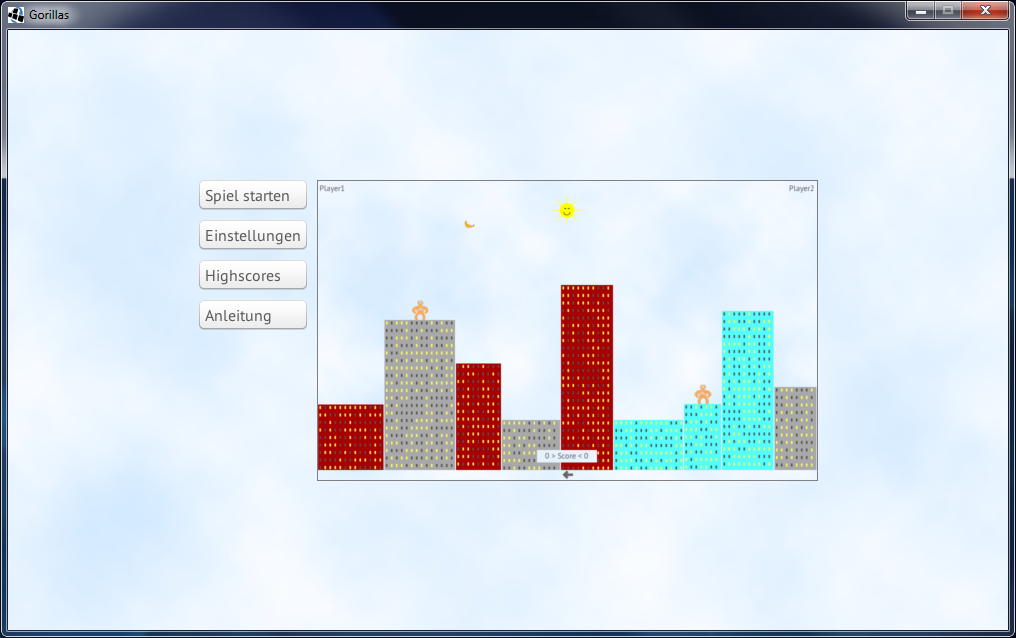
\includegraphics[scale=0.4]{\basepath/\shortGameTitle/menu.png}
\caption{Beispiel einer grafischen Umsetzung des Menüs von \gameTitle}
\label{fig:screenshot1}
\end{center}
\end{figure}

\begin{figure}[htb]
\begin{center}
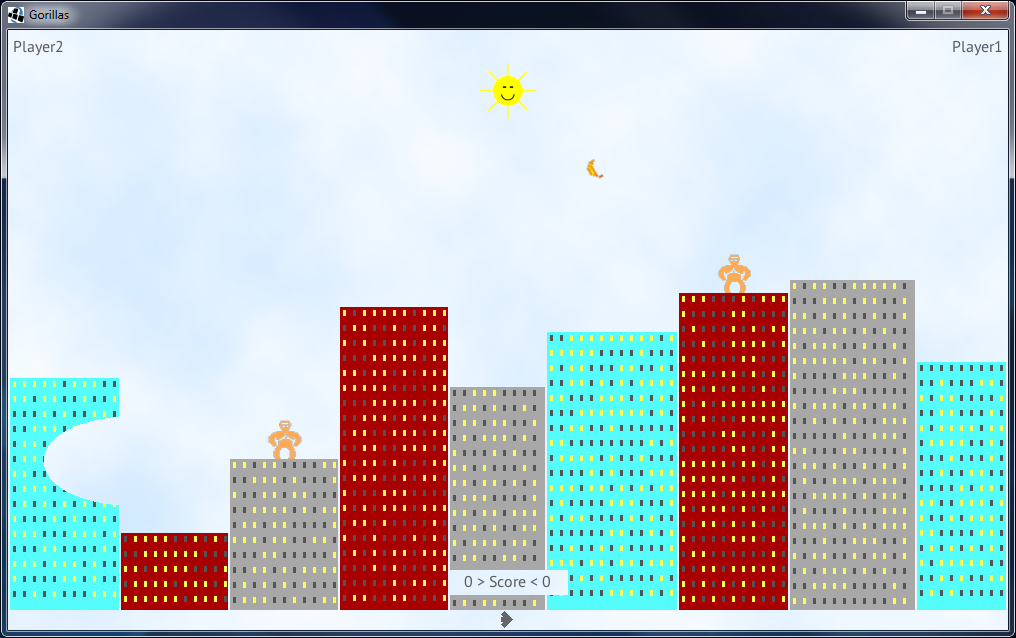
\includegraphics[scale=.4]{\basepath/\shortGameTitle/gameplay.png}
\caption{Beispiel einer grafischen Umsetzung des Spielfensters von \gameTitle}
\label{fig:screenshot2}
\end{center}
\end{figure}
